\chapter{Introduction}
\hypertarget{chapter:introduction}{}

This project addresses a pressing challenge in the evolution of gaming experiences: how to adapt and extend the social and immersive qualities of local multiplayer systems -- exemplified by the Nintendo Wii -- to a modern, online environment. The Nintendo Wii has gained a large and dedicated following due to its motion controls, comparatively low price, and its local multiplayer gameplay. However, as online gaming has become the norm\cite{businesswireOnlineGaming}, the traditional split-screen and communal experiences that defined the Wii era have faced diminishing support and new technical challenges. The main challenge is that, due to the termination of first party online services\cite{nintendoTerminationNintendo}, the Wii no longer supports online multiplayer. This coupled with the fact that most people no longer play multiplayer games locally\cite{academyofanimatedartOnlineGaming}, means that the Wii’s local multiplayer games are no longer accessible to a large portion of its possible player base.

This project aims to address this issue by developing a system that enables remote players to experience the Wii’s local multiplayer games in an online setting. At a high level, the system allows a remote ``client'' user to interface with a Wii console over a network connection while a local ``host'' user interfaces with the Wii console over a native Bluetooth connection as shown in Figure~\ref{fig:simple_overview}.

\begin{figure}[h]
	\centering
	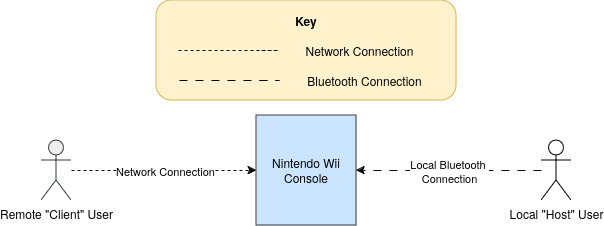
\includegraphics[width=1\textwidth]{simple_intro.jpg}
	\caption{Simple Overview of the System}
	\label{fig:simple_overview}
\end{figure}

However, this simple overview does not capture the complexity of the system. The remote user needs to be able to see and hear the game as well as use a physical Wii Remote to control the game. The system -- as shown in Figure~\ref{fig:expanded_overview} -- consists of three main components: a capture and streaming system, a controller input relay system, and a Wii Remote emulator. The capture and streaming system is responsible for capturing the Wii’s video and audio output and streaming it to remote players through the host machine. The controller input relay system transmits the Wii Remote’s controller data from the client machine to the host machine over a low-latency network connection. The Wii Remote emulator, running on the host machine, receives the controller data and emulates the remote user's Wii Remote input.

\begin{figure}[ht]
	\centering
	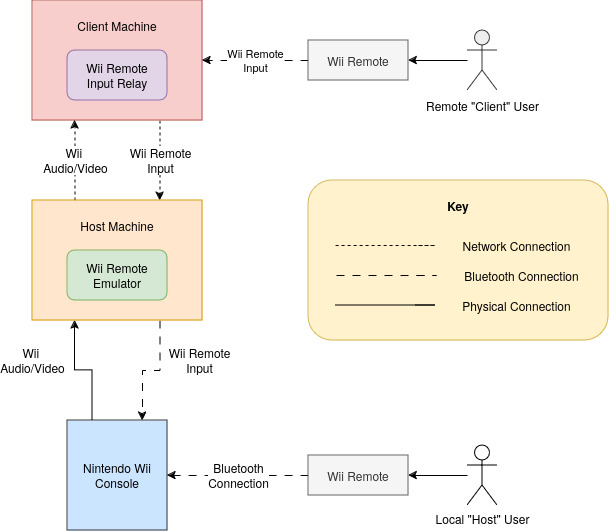
\includegraphics[width=1\textwidth]{advanced_intro.jpg}
	\caption{System Architecture and Data Flow}
	\label{fig:expanded_overview}
\end{figure}

The key objectives of the project are to:
\begin{enumerate}
	\item  Develop a system to capture and stream the Wii’s video and audio output to remote players.
	\item Develop a system to relay the Wii Remote’s controller data over a low-latency network connection.
	\item Evaluate the system’s performance and user experience in a real-world setting.
\end{enumerate}

This report will introduce discussions of the technical design, implementation challenges, and testing procedures that collectively contribute to a solution aimed at revitalising retro gaming experiences. The subsequent chapters present an in-depth analysis of the system architecture, design decisions, and the experimental validation of the proposed solution.
